\documentclass[conference]{IEEEtran}
\usepackage{cite}
\usepackage{amsmath,amssymb}
\usepackage{graphicx}
\usepackage{booktabs}
\usepackage{url}
\usepackage{tikz}
\usetikzlibrary{arrows.meta,positioning}
\usepackage[hidelinks]{hyperref}
\hypersetup{
  colorlinks=true,
  linkcolor=blue,
  citecolor=blue,
  urlcolor=blue,
  pdftitle={X-Fusion: An Engineering Prototype for Tri-Modal Chest Radiograph Analysis},
  pdfauthor={P. Deepesh Reddy, R. Vignesh, R. Sidhardh Reddy, Saharsh Machendra, V. Surya Venkat, K. Vishal Reddy}
}

\begin{document}

\title{X-Fusion: An Engineering Prototype for Tri-Modal Chest Radiograph Analysis}

\author{\IEEEauthorblockN{P. Deepesh Reddy, R. Vignesh, R. Sidhardh Reddy, Saharsh Machendra, V. Surya Venkat, and K. Vishal Reddy}
\IEEEauthorblockA{Department of Computer Science and Engineering\\
Keshav Memorial Institute of Technology\\
Hyderabad, Telangana, India\\
Email: \texttt{Kasarlavishalreddy@gmail.com}}}

\maketitle

\begin{abstract}
Chest radiograph interpretation is performed alongside clinical history and patient measurements, while many automated systems operate on images alone. This paper documents X-Fusion, a research prototype that accepts a chest radiograph, a free-text note, and six structured fields (age, sex, temperature, heart rate, respiratory rate, and oxygen saturation) and returns scores for fourteen findings. The implementation combines a pretrained BiomedCLIP image encoder, a CXR-BERT text encoder, a metadata multilayer perceptron, and a two-layer Transformer encoder over three modality tokens and a learned classification token. A FastAPI inference service and a Next.js browser interface expose the model and its exploratory explanation outputs. Inspection of the training pipeline reveals a central validity limitation: report text and four vital signs are generated from the same disease labels used as prediction targets. This creates direct target leakage, so validation loss and checkpoint outputs cannot establish diagnostic performance or independent value from the auxiliary modalities. The saved training trace records decreasing losses over fourteen logged epochs, but the repository contains no auditable per-class test evaluation that resolves this leakage. We therefore present X-Fusion as an implementation and workflow prototype, not a clinically validated decision-support system.
\end{abstract}

\begin{IEEEkeywords}
Chest radiography, multimodal learning, medical image analysis, Transformer, multi-label classification, data leakage, explainable AI.
\end{IEEEkeywords}

\section{Introduction}
Chest radiographs are widely used to assess pulmonary and cardiothoracic findings. Public datasets such as NIH ChestX-ray14 and CheXpert have supported large-scale research into automated chest radiograph classification \cite{wang2017,irvin2019}. At the same time, radiological interpretation is contextual: symptoms, imaging indications, patient history, and measurements can influence how an image is understood. This motivates research into systems that can represent more than image pixels.

X-Fusion is a software prototype for exploring that input pattern. It accepts an image, a clinical note, and structured patient values, encodes these inputs separately, and combines their representations for fourteen-label prediction. The repository also includes a model-serving API, a browser-based interface, an attention visualization, and metadata attribution code. This paper reports what is implemented and what can be substantiated from the available artifacts; it does not claim a new clinical method or a performance improvement over prior work.

An important qualification emerged from examining the data path. The current dataset class creates report-like text from the target disease labels and samples four vital signs using distributions conditioned on those labels. Since the same labels supervise the prediction head, these auxiliary inputs contain target-derived information. This leakage invalidates clinical interpretations of the observed losses and predictions. We make this limitation explicit and avoid reporting unsupported diagnostic metrics.

The contributions of this paper are therefore limited and implementation-focused:
\begin{itemize}
  \item We describe the implemented image, text, and structured-data encoders and their Transformer-based fusion path.
  \item We document the training and serving components and the available optimization evidence.
  \item We identify the label-derived auxiliary inputs as a direct threat to evaluation validity and state the evidence required before a clinical performance study can be claimed.
\end{itemize}

\section{Related Work}
\subsection{Chest Radiograph Classification}
The NIH ChestX-ray8 release introduced a large chest radiograph collection with labels for thoracic findings; the later ChestX-ray14 benchmark is commonly associated with fourteen labels \cite{wang2017}. CheXpert provides a separate dataset with uncertainty labels and an expert-labelled evaluation subset \cite{irvin2019}. Both works establish the context for multi-label chest radiograph studies, but a benchmark name alone does not demonstrate that a particular implementation used the complete dataset or produced valid evaluation results. X-Fusion uses the NIH metadata and split lists available in the project workspace and filters records to image files present locally.

\subsection{Vision and Language Encoders}
The Vision Transformer (ViT) models an image as a sequence of patches processed with self-attention \cite{dosovitskiy2021}. BiomedCLIP is a biomedical vision-language model pretrained on scientific image-text pairs \cite{biomedclip2023}. CXR-BERT provides a language model specialized for chest radiology text \cite{cxrbert2022}. X-Fusion uses these pretrained components as modality encoders. Its training notes, however, are synthesized from labels rather than being paired clinical reports; therefore, the text branch should not be interpreted as evidence that real report context improves prediction.

\subsection{Optimization and Explanations}
Asymmetric Loss (ASL) modifies the contribution of positive and negative labels and has been proposed for multi-label imbalance \cite{ridnik2021}. Contrastive learning objectives such as InfoNCE train matched representations to score above mismatched examples \cite{oord2018}. SHAP provides a framework for feature attribution using Shapley values \cite{lundberg2017}. Attention visualizations can expose model-internal weights, but an attention map alone is not a validated lesion-localization method or a causal explanation \cite{chefer2021}. The corresponding X-Fusion outputs are exploratory inspection aids, not clinically validated explanations.

\section{System Overview}
The project contains a Python backend and a Next.js frontend. The browser interface supports image selection, entry of a note and patient values, preset example cases, prediction display, and session-local case history. It sends a multipart request to the FastAPI \texttt{/predict} endpoint. The backend loads a checkpoint at startup, preprocesses the uploaded image, invokes the model, and returns class scores together with an attention overlay and, when available, metadata attributions. The \texttt{/health} endpoint reports model readiness.

\begin{figure*}[t]
\centering
\resizebox{0.96\textwidth}{!}{%
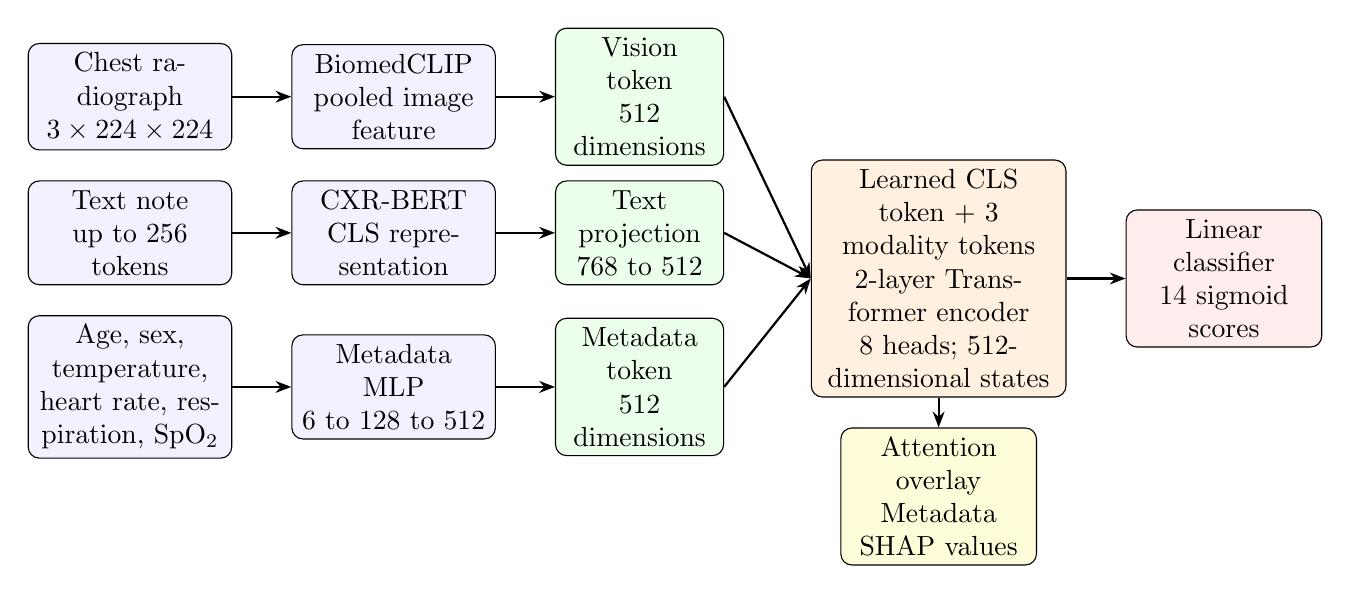
\begin{tikzpicture}[
  node distance=0.65cm and 0.75cm,
  box/.style={draw,rounded corners,align=center,minimum height=0.82cm,text width=2.35cm,fill=blue!5},
  token/.style={draw,rounded corners,align=center,minimum height=0.75cm,text width=1.9cm,fill=green!8},
  fusion/.style={draw,rounded corners,align=center,minimum height=1.15cm,text width=3.0cm,fill=orange!12},
  output/.style={draw,rounded corners,align=center,minimum height=0.9cm,text width=2.25cm,fill=red!7},
  arr/.style={-{Stealth[length=2mm]},thick}
]
\node[box] (image) {Chest radiograph\\$3 \times 224 \times 224$};
\node[box,right=of image] (vision) {BiomedCLIP\\pooled image feature};
\node[token,right=of vision] (vtoken) {Vision token\\512 dimensions};
\node[box,below=0.38cm of image] (note) {Text note\\up to 256 tokens};
\node[box,right=of note] (text) {CXR-BERT\\CLS representation};
\node[token,right=of text] (ttoken) {Text projection\\768 to 512};
\node[box,below=0.38cm of note] (meta) {Age, sex, temperature,\\heart rate, respiration, SpO$_2$};
\node[box,right=of meta] (mlp) {Metadata MLP\\6 to 128 to 512};
\node[token,right=of mlp] (mtoken) {Metadata token\\512 dimensions};
\node[fusion,right=1.1cm of ttoken,yshift=-0.58cm] (transformer) {Learned CLS token + 3 modality tokens\\2-layer Transformer encoder\\8 heads; 512-dimensional states};
\node[output,right=of transformer] (head) {Linear classifier\\14 sigmoid scores};
\node[output,below=0.38cm of transformer,fill=yellow!15] (explain) {Attention overlay\\Metadata SHAP values};
\draw[arr] (image) -- (vision);
\draw[arr] (vision) -- (vtoken);
\draw[arr] (note) -- (text);
\draw[arr] (text) -- (ttoken);
\draw[arr] (meta) -- (mlp);
\draw[arr] (mlp) -- (mtoken);
\draw[arr] (vtoken.east) -- (transformer.west);
\draw[arr] (ttoken.east) -- (transformer.west);
\draw[arr] (mtoken.east) -- (transformer.west);
\draw[arr] (transformer) -- (head);
\draw[arr] (transformer) -- (explain);
\end{tikzpicture}%
}
\caption{Implemented inference path. The fusion block is a Transformer encoder applying self-attention to the four-token sequence; the name of its source class does not imply a separate cross-attention mechanism.}
\label{fig:architecture}
\end{figure*}

\section{Model}
\subsection{Modality Encoders}
The image is resized to $224 \times 224$ pixels, converted to RGB, and normalized using the channel means and standard deviations in the implementation. The visual encoder is the ViT-B/16 model selected through OpenCLIP's BiomedCLIP Hugging Face identifier. Its pooled 512-dimensional image representation is retained as one token.

The text branch tokenizes each note with the \url{microsoft/BiomedVLP-CXR-BERT-specialized} tokenizer, truncating to 256 tokens. The first hidden-state vector is projected from the encoder's 768-dimensional representation to 512 dimensions. The metadata vector is
\[
\mathbf{m} =
[\text{age},\text{sex},\text{temperature},\text{heart rate},
\text{respiratory rate},\text{SpO}_2],
\]
and is transformed by a two-layer MLP with a 128-unit hidden layer into a 512-dimensional token. Continuous metadata is not normalized by a learned training-set normalization step in the current data pipeline.

\subsection{Token Fusion and Prediction}
Let $\mathbf{v}_i$, $\mathbf{t}_i$, and $\mathbf{m}_i$ denote the image, text, and metadata token for example $i$. A learned token $\mathbf{c}$ is prepended to form
\[
\mathbf{Z}_i = [\mathbf{c};\mathbf{v}_i;\mathbf{t}_i;\mathbf{m}_i].
\]
The code applies a two-layer Transformer encoder with eight attention heads, model width 512, feed-forward width 2048, GELU activation, and dropout 0.1. Thus, interactions occur through self-attention over the four-token sequence, rather than through an explicitly separate cross-attention block. The encoded CLS position $\mathbf{h}_i$ is passed to a dropout-and-linear head:
\[
\mathbf{z}_i = \mathbf{W}\,\mathrm{Dropout}(\mathbf{h}_i)+\mathbf{b},
\qquad
\hat{\mathbf{y}}_i = \sigma(\mathbf{z}_i)\in[0,1]^{14}.
\]
Each output is an independent sigmoid score for one of the fourteen NIH finding labels. The serving code ranks these scores and applies a 0.30 cutoff to the maximum score to select its displayed summary status. This application-level cutoff is not a threshold calibrated on a held-out clinical dataset.

\subsection{Training Objective}
The Lightning module computes ASL for the fourteen labels. For logit $z_{ic}$ and target $y_{ic}$, let $p_{ic}=\sigma(z_{ic})$ and $\tilde{p}_{ic}=\min(1,1-p_{ic}+0.05)$. The implemented classification loss is
\begin{equation}
\begin{aligned}
\mathcal{L}_{\mathrm{ASL}} =
-\frac{1}{B}\sum_{i=1}^{B}\sum_{c=1}^{14}
\Bigl(&y_{ic}\log(p_{ic})(1-p_{ic})^{\gamma_+}\\
&+(1-y_{ic})\log(\tilde{p}_{ic})(1-\tilde{p}_{ic})^{\gamma_-}\Bigr),
\end{aligned}
\label{eq:asl}
\end{equation}
with $\gamma_+=1$ and $\gamma_-=4$. The code also computes symmetric image--text InfoNCE. For normalized image and text embeddings, $s_{ij}=\mathbf{v}_i^\top\mathbf{t}_j/\tau$, with $\tau=0.07$, and
\begin{equation}
\mathcal{L}_{\mathrm{NCE}} =
\frac{1}{2}\left[
\mathrm{CE}(S,I_B)+\mathrm{CE}(S^\top,I_B)
\right],
\label{eq:nce}
\end{equation}
where $I_B$ denotes the diagonal pairing of examples in a batch. The total training loss is
\begin{equation}
\mathcal{L}_{\mathrm{train}} =
\mathcal{L}_{\mathrm{ASL}}+0.1\,\mathcal{L}_{\mathrm{NCE}}.
\label{eq:total}
\end{equation}
Validation loss is ASL alone. Accordingly, the two logged loss curves are not directly comparable as measurements of the same objective.

\subsection{Explanation Outputs}
The image visualization hooks the query-key-value projection in the final visual Transformer block, computes attention weights, averages the CLS-to-patch weights across heads, reshapes the 196 patch values to a $14 \times 14$ map, and overlays the resized heatmap on the input. This is an attention visualization, not a gradient-based class explanation or validated localization map.

The metadata explanation uses Kernel SHAP while holding image and text features fixed. The implementation takes absolute attribution magnitudes and aggregates across output labels before normalization. It therefore represents aggregate relative metadata attribution, not signed, class-specific effects. Both explanation paths require independent validation before they can support clinical interpretation.

\section{Data and Experimental Setup}
\subsection{Dataset and Partitioning}
The data module reads the NIH ChestX-ray14 metadata CSV and its official train/validation and test image lists. It first filters metadata records to PNG images available in the local image directory. The official train/validation pool is then divided by patient identifier: the code shuffles the unique patient identifiers using NumPy seed 42 and assigns 10\% of those identifiers to validation. The official test list is used for the test partition. This procedure is intended to keep patients separated between train and validation and relies on the official list for the held-out test assignment.

In the inspected workspace snapshot, the metadata CSV contained 112,120 records and 31,877 local PNG files. Of the CSV records, 31,630 had a matching local image: 24,530 appeared in the official train/validation list and 7,100 in the official test list. These counts describe the available local subset, not a full-dataset experiment.

\begin{table}[t]
\caption{Locally Available Images Matched to the Metadata CSV}
\label{tab:localdata}
\centering
\scriptsize
\begin{tabular}{lr}
\toprule
Partition before patient-level validation split & Images \\
\midrule
Official train/validation pool & 24,530 \\
Official test list & 7,100 \\
\midrule
Total matched local images & 31,630 \\
\bottomrule
\end{tabular}
\end{table}

Training images receive random horizontal flipping, rotation up to ten degrees, and brightness and contrast jitter. Validation and test images are resized and normalized without these random image augmentations. The label vector contains fourteen multi-hot findings. Age and sex are read from the metadata CSV; the other four structured fields are synthesized.

\subsection{Label-Derived Inputs and Evaluation Validity}
The data class constructs each text note by selecting report templates associated with the disease labels for that image. It also samples temperature, heart rate, respiratory rate, and oxygen saturation from distributions selected according to label conditions, including pneumonia and edema. The same label vector is used as the supervised target. Therefore, information derived from the target enters both the text and metadata branches before prediction. The generated values are not independent clinical observations, and the notes are not real radiology reports paired with the images.

This relationship is shown in Fig.~\ref{fig:leakage}. It creates direct target leakage. Consequently, validation losses and any metrics computed on these generated modalities cannot be used as evidence of clinical generalization or of benefit from multimodal inputs. The data loader also samples report variants and vital signs when examples are accessed, so these auxiliary inputs may differ between passes. A valid follow-up study requires genuinely paired, time-aligned, independently collected clinical notes and measurements, with patient-level partitions and a reproducible evaluation protocol.

\begin{figure}[t]
\centering
\resizebox{\columnwidth}{!}{%
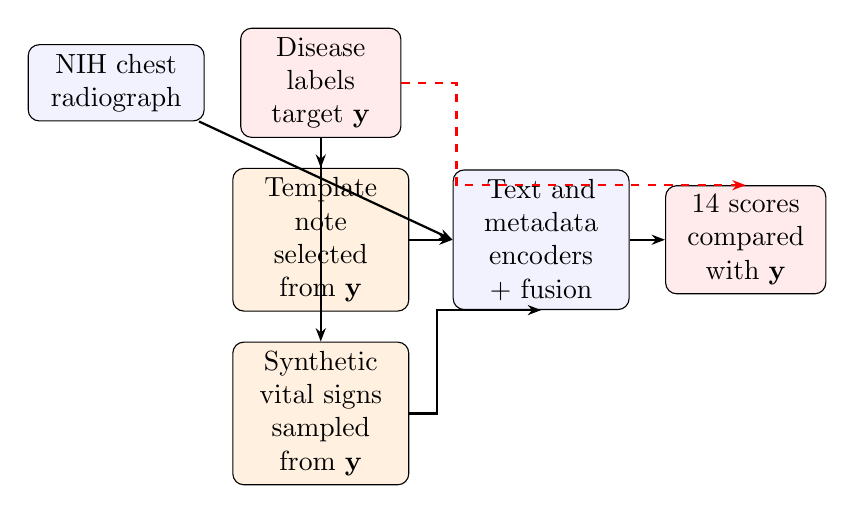
\begin{tikzpicture}[
  node distance=0.38cm and 0.45cm,
  box/.style={draw,rounded corners,align=center,minimum height=0.78cm,text width=2.0cm,fill=blue!5},
  generated/.style={draw,rounded corners,align=center,minimum height=0.78cm,text width=2.0cm,fill=orange!12},
  label/.style={draw,rounded corners,align=center,minimum height=0.78cm,text width=1.8cm,fill=red!8},
  arr/.style={-{Stealth[length=1.7mm]},thick},
  leak/.style={-{Stealth[length=1.7mm]},thick,dashed,red}
]
\node[box] (image) {NIH chest radiograph};
\node[label,right=of image] (target) {Disease labels\\target $\mathbf{y}$};
\node[generated,below=of target] (note) {Template note\\selected from $\mathbf{y}$};
\node[generated,below=of note] (vitals) {Synthetic vital signs\\sampled from $\mathbf{y}$};
\node[box,right=of note,xshift=0.1cm] (model) {Text and metadata\\encoders + fusion};
\node[label,right=of model] (prediction) {14 scores\\compared with $\mathbf{y}$};
\draw[arr] (image) -- (model.west);
\draw[arr] (target) -- (note);
\draw[arr] (target) -- (vitals);
\draw[arr] (note) -- (model);
\draw[arr] (vitals.east) -- ++(0.35,0) |- (model.south);
\draw[arr] (model) -- (prediction);
\draw[leak] (target.east) -- ++(0.7,0) |- (prediction.north);
\end{tikzpicture}%
}
\caption{Training-data dependency in the current implementation. The dashed path emphasizes that target-derived labels generate two model inputs as well as supervising the output.}
\label{fig:leakage}
\end{figure}

\subsection{Training Configuration}
The advanced laptop training script configures a batch size of 4, gradient accumulation over 8 batches, a maximum of 15 epochs, mixed-precision training, learning rate $2\times10^{-4}$, and weight decay $10^{-4}$. It freezes the text encoder and attempts to leave the final two visual Transformer blocks trainable. The checkpoint hyperparameters record the learning rate, weight decay, modality dimension, and encoder freeze flags. Since selective unfreezing depends on parameter names in the installed OpenCLIP implementation, the exact trainable parameter set should be recorded when reproducing the run.

\begin{table}[t]
\caption{Selected Implementation and Run Settings}
\label{tab:settings}
\centering
\scriptsize
\begin{tabular}{p{0.30\columnwidth}p{0.57\columnwidth}}
\toprule
Component & Implemented setting \\
\midrule
Image input & RGB, $224 \times 224$ pixels \\
Image feature & BiomedCLIP pooled vector, 512 dimensions \\
Text feature & CXR-BERT CLS, projected 768 to 512 \\
Metadata & Six inputs; MLP 6 to 128 to 512 \\
Fusion & Learned CLS + 3 modality tokens; 2 layers; 8 heads \\
Output & 14 independent sigmoid scores \\
Loss & ASL + 0.1 InfoNCE; $\tau=0.07$ \\
Advanced run & Batch 4; accumulation 8; max 15 epochs \\
Optimizer & AdamW; cosine annealing scheduler \\
\bottomrule
\end{tabular}
\end{table}

\section{Results and Discussion}
The saved TensorBoard event artifact contains fourteen logged epoch-level values for the advanced run. The plotted training objective decreases from 0.1545 to 0.1190, while validation ASL decreases from 0.0207 to 0.0007 (Fig.~\ref{fig:loss}). These are recorded optimization values, not estimates of diagnostic accuracy. The training objective includes the contrastive term; validation loss does not. More importantly, both curves are obtained under the label-derived auxiliary-input pipeline described above. Their decline cannot establish patient-independent predictive performance.

\begin{figure}[t]
\centering
\includegraphics[width=\columnwidth]{../../paper_assets/fig4_training_trace.png}
\caption{Recorded training objective and validation classification loss over fourteen logged epochs. The input pipeline derives synthetic notes and vital signs from the target labels; this plot is not a clinical performance evaluation.}
\label{fig:loss}
\end{figure}

The repository includes evaluation code that can log multi-label accuracy and AUROC, but the available project artifacts do not provide a reproducible per-class test prediction file or a trustworthy held-out metric report that resolves the leakage. We therefore omit claims of AUROC, average precision, sensitivity, specificity, calibration, statistical significance, state-of-the-art performance, or improvement over an image-only baseline. Results in an older draft that lack a verifiable evaluation artifact should not be treated as measured outcomes.

The application demonstrates that the image, note, and metadata can be passed through a local inference interface and that prediction and explanation outputs are wired into a web workflow. Such software functionality is distinct from clinical utility. In particular, a checkpoint loading successfully or a request returning scores would not validate those scores as calibrated diagnoses.

\section{Limitations and Responsible Use}
The principal limitation is target leakage from label-conditioned notes and vital signs. Other limitations are the incomplete local image subset, stochastic synthetic auxiliary values, absence of continuous-metadata normalization, and lack of an auditable external or prospective evaluation. The visual branch supplies a pooled image embedding to fusion rather than exposing patch tokens to the multimodal Transformer. The selective vision fine-tuning behavior is dependent on parameter-name matching and should be verified for any reproduction. The application-level decision cutoff has not been clinically calibrated.

The system is a research prototype and is not a medical device. Its scores, attention visualization, and metadata attributions must not be used to diagnose, triage, or guide patient care. A credible clinical study would require independent paired inputs, a frozen patient-disjoint test set, per-class discrimination and calibration measures with confidence intervals, documented thresholds, external validation, and review by qualified clinicians. Data governance, privacy, and security controls would also be required before deployment with patient information.

\section{Conclusion}
This paper documents X-Fusion as implemented: three modality encoders, a four-token Transformer encoder, a fourteen-output classifier, explanation utilities, a FastAPI service, and a Next.js client. The project provides an end-to-end engineering workflow and a saved optimization trace. However, the current dataset pipeline generates reports and vital signs from the supervised findings, making the auxiliary modalities label-dependent. No clinical performance claim can be supported from the available training trace. Replacing those synthetic inputs with independent, paired clinical data and producing a reproducible patient-level test evaluation are necessary steps before assessing diagnostic value.

\section*{Acknowledgment}
The authors thank K. Vishal Reddy for mentorship and project guidance. The NIH ChestX-ray14 dataset is acknowledged as the source of the image metadata and labels used by the project data pipeline.

\begin{thebibliography}{00}
\bibitem{wang2017}
X. Wang, Y. Peng, L. Lu, Z. Lu, M. Bagheri, and R. M. Summers, ``ChestX-ray8: Hospital-scale chest X-ray database and benchmarks on weakly-supervised classification and localization of common thorax diseases,'' in \emph{Proc. IEEE Conf. Comput. Vis. Pattern Recognit.}, 2017, pp. 2097--2106, doi: 10.1109/CVPR.2017.369.

\bibitem{irvin2019}
J. Irvin \emph{et al.}, ``CheXpert: A large chest radiograph dataset with uncertainty labels and expert comparison,'' in \emph{Proc. AAAI Conf. Artif. Intell.}, vol. 33, 2019, pp. 590--597, doi: 10.1609/aaai.v33i01.3301590.

\bibitem{dosovitskiy2021}
A. Dosovitskiy \emph{et al.}, ``An image is worth 16x16 words: Transformers for image recognition at scale,'' in \emph{Proc. Int. Conf. Learn. Represent.}, 2021.

\bibitem{biomedclip2023}
S. Zhang \emph{et al.}, ``BiomedCLIP: A multimodal biomedical foundation model pretrained on fifteen million scientific image-text pairs,'' arXiv:2303.00915, 2023.

\bibitem{cxrbert2022}
B. Boecking \emph{et al.}, ``Making the most of text semantics to improve biomedical vision-language models,'' in \emph{Computer Vision -- ECCV 2022}, 2022.

\bibitem{ridnik2021}
T. Ridnik, E. Ben-Baruch, A. Noy, and L. Zelnik-Manor, ``Asymmetric loss for multi-label classification,'' in \emph{Proc. IEEE/CVF Int. Conf. Comput. Vis.}, 2021, pp. 82--91, doi: 10.1109/ICCV48922.2021.00014.

\bibitem{oord2018}
A. van den Oord, Y. Li, and O. Vinyals, ``Representation learning with contrastive predictive coding,'' arXiv:1807.03748, 2018.

\bibitem{lundberg2017}
S. M. Lundberg and S.-I. Lee, ``A unified approach to interpreting model predictions,'' in \emph{Advances in Neural Information Processing Systems}, vol. 30, 2017.

\bibitem{chefer2021}
H. Chefer, S. Gur, and L. Wolf, ``Transformer interpretability beyond attention visualization,'' in \emph{Proc. IEEE/CVF Conf. Comput. Vis. Pattern Recognit.}, 2021, pp. 782--791, doi: 10.1109/CVPR46437.2021.00084.

\bibitem{nihdataset}
National Institutes of Health Clinical Center, ``ChestX-ray14 dataset.'' [Online]. Available: \url{https://nihcc.app.box.com/v/ChestXray-Nihcc}
\end{thebibliography}

\end{document}
